\section{Задача 2.17}
\subsection{Задание:}
Вычислить ранг матрицы $ A =
	\begin{pmatrix}
			11 & 0 & 11 & 8 & 0 & 4 & 8 \\
			15 & 0 & 0 & -3 & -15 & 0 & -6 \\
			13 & -9 & 0 & 14 & 0 & 10 & 0 \\
			-1 & 0 & -7 & 0 & 12 & -15 & 14 \\
			-7 & 0 & -2 & 0 & 0 & 12 & 0 \\
	\end{pmatrix}
$
\subsection{Решение:}
Приведём матрицу $ A $ к ступенчатому виду с помощю элементарных преобразований:
\\
$
\begin{pmatrix}
	11 & 0 & 11 & 8 & 0 & 4 & 8 \\
	15 & 0 & 0 & -3 & -15 & 0 & -6 \\
	13 & -9 & 0 & 14 & 0 & 10 & 0 \\
	-1 & 0 & -7 & 0 & 12 & -15 & 14 \\
	-7 & 0 & -2 & 0 & 0 & 12 & 0 \\
\end{pmatrix}
\sim
\begin{pmatrix}
	15 & 0 & 0 & -3 & -15 & 0 & -6 \\
	11 & 0 & 11 & 8 & 0 & 4 & 8 \\
	13 & -9 & 0 & 14 & 0 & 10 & 0 \\
	-1 & 0 & -7 & 0 & 12 & -15 & 14 \\
	-7 & 0 & -2 & 0 & 0 & 12 & 0 \\
\end{pmatrix}
\sim
\\
\begin{pmatrix}
	15 & 0 & 0 & -3 & -15 & 0 & -6 \\
	0 & 0 & 11 & \frac{51}{5} & 11 & 4 & \frac{62}{5} \\
	13 & -9 & 0 & 14 & 0 & 10 & 0 \\
	-1 & 0 & -7 & 0 & 12 & -15 & 14 \\
	-7 & 0 & -2 & 0 & 0 & 12 & 0 \\
\end{pmatrix}
\sim
\begin{pmatrix}
	5 & 0 & 0 & -1 & -5 & 0 & -2 \\
	0 & 0 & 11 & \frac{51}{5} & 11 & 4 & \frac{62}{5} \\
	13 & -9 & 0 & 14 & 0 & 10 & 0 \\
	-1 & 0 & -7 & 0 & 12 & -15 & 14 \\
	-7 & 0 & -2 & 0 & 0 & 12 & 0 \\
\end{pmatrix}
\sim
\\
\begin{pmatrix}
	5 & 0 & 0 & -1 & -5 & 0 & -2 \\
	0 & 0 & 55 & 51 & 55 & 20 & 62 \\
	13 & -9 & 0 & 14 & 0 & 10 & 0 \\
	-1 & 0 & -7 & 0 & 12 & -15 & 14 \\
	-7 & 0 & -2 & 0 & 0 & 12 & 0 \\
\end{pmatrix}
\sim
\begin{pmatrix}
	5 & 0 & 0 & -1 & -5 & 0 & -2 \\
	0 & 0 & 55 & 51 & 55 & 20 & 62 \\
	0 & -9 & 0 & \frac{83}{5} & 13 & 10 & \frac{26}{5} \\
	-1 & 0 & -7 & 0 & 12 & -15 & 14 \\
	-7 & 0 & -2 & 0 & 0 & 12 & 0 \\
\end{pmatrix}
\sim
\\
\begin{pmatrix}
	5 & 0 & 0 & -1 & -5 & 0 & -2 \\
	0 & 0 & 55 & 51 & 55 & 20 & 62 \\
	0 & -45 & 0 & 83 & 65 & 50 & 26 \\
	-1 & 0 & -7 & 0 & 12 & -15 & 14 \\
	-7 & 0 & -2 & 0 & 0 & 12 & 0 \\
\end{pmatrix}
\sim
\begin{pmatrix}
	5 & 0 & 0 & -1 & -5 & 0 & -2 \\
	0 & 0 & 55 & 51 & 55 & 20 & 62 \\
	0 & -45 & 0 & 83 & 65 & 50 & 26 \\
	0 & 0 & -7 & -\frac{1}{5} & 11 & -15 & \frac{68}{5} \\
	-7 & 0 & -2 & 0 & 0 & 12 & 0 \\
\end{pmatrix}
\sim
\\
\begin{pmatrix}
	5 & 0 & 0 & -1 & -5 & 0 & -2 \\
	0 & 0 & 55 & 51 & 55 & 20 & 62 \\
	0 & -45 & 0 & 83 & 65 & 50 & 26 \\
	0 & 0 & 35 & 1 & -55 & 75 & -68 \\
	-7 & 0 & -2 & 0 & 0 & 12 & 0 \\
\end{pmatrix}
\sim
\begin{pmatrix}
	5 & 0 & 0 & -1 & -5 & 0 & -2 \\
	0 & 0 & 55 & 51 & 55 & 20 & 62 \\
	0 & -45 & 0 & 83 & 65 & 50 & 26 \\
	0 & 0 & 35 & 1 & -55 & 75 & -68 \\
	0 & 0 & -2 & -\frac{7}{5} & -7 & 12 & -\frac{14}{5} \\
\end{pmatrix}
\sim
\\
\begin{pmatrix}
	5 & 0 & 0 & -1 & -5 & 0 & -2 \\
	0 & 0 & 55 & 51 & 55 & 20 & 62 \\
	0 & -45 & 0 & 83 & 65 & 50 & 26 \\
	0 & 0 & 35 & 1 & -55 & 75 & -68 \\
	0 & 0 & 10 & 7 & 35 & -60 & 14 \\
\end{pmatrix}
\sim
\begin{pmatrix}
	5 & 0 & 0 & -1 & -5 & 0 & -2 \\
	0 & -45 & 0 & 83 & 65 & 50 & 26 \\
	0 & 0 & 55 & 51 & 55 & 20 & 62 \\
	0 & 0 & 35 & 1 & -55 & 75 & -68 \\
	0 & 0 & 10 & 7 & 35 & -60 & 14 \\
\end{pmatrix}
\sim
\\
\begin{pmatrix}
	5 & 0 & 0 & -1 & -5 & 0 & -2 \\
	0 & 45 & 0 & -83 & -65 & -50 & -26 \\
	0 & 0 & 55 & 51 & 55 & 20 & 62 \\
	0 & 0 & 0 & 346 & 990 & -685 & 1182 \\
	0 & 0 & 10 & 7 & 35 & -60 & 14 \\
\end{pmatrix}
\sim
\begin{pmatrix}
	5 & 0 & 0 & -1 & -5 & 0 & -2 \\
	0 & 45 & 0 & -83 & -65 & -50 & -26 \\
	0 & 0 & 55 & 51 & 55 & 20 & 62 \\
	0 & 0 & 0 & 346 & 990 & -685 & 1182 \\
	0 & 0 & 0 & -5 & 55 & -140 & 6 \\
\end{pmatrix}
\sim
\\
\begin{pmatrix}
	5 & 0 & 0 & -1 & -5 & 0 & -2 \\
	0 & 45 & 0 & -83 & -65 & -50 & -26 \\
	0 & 0 & 55 & 51 & 55 & 20 & 62 \\
	0 & 0 & 0 & 346 & 990 & -685 & 1182 \\
	0 & 0 & 0 & 0 & 2180 & -4715 & 726 \\
\end{pmatrix}
$
\\
Из приведённой к ступенчатому виду матрицы видно что $ rank A = 51 $.
\subsection{Выполним компьютерную проверку в среде Wolfram Mathematica:}
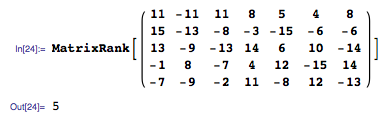
\includegraphics[scale=0.6]{task/2_17/screen.png}
